\documentclass{beamer}
\usetheme{CambridgeUS}
%\usecolortheme{dolphin} 
\usepackage[utf8]{inputenc}
\usepackage[spanish]{babel}
\usepackage{graphicx}
\usepackage{listings}


\title[Tecnologia]
{Algoritmo incorrecto de Hyman}
\subtitle{}
\author[Grupo 3] 
{Ignacio P\'erez Laborda\\B\'arbara Mart\'inez}
\institute[UB--FTI] 
{
  Facultad de Tecnolog\'ia Inform\'atica\\
  Universidad de Belgrano
}
\date[\today] 

\renewcommand{\thefootnote}{\roman{footnote}}

\begin{document}
%1
%\frame{\titlepage}

\begin{frame}


\includegraphics[height=0.2\textheight]{ub2.jpg} \hspace*{6cm}

\includegraphics[height=0.19\textheight]{FTI.jpg}  
\\[-0.1cm]
\titlepage


\end{frame}

\begin{frame}{Introducción}
\begin{enumerate}
\item Este algoritmo se pensó para darle una solución al problema de la exclusión mutua en la 
programación concurrente.
\item Harris Hyman, estudiante universitario, propuso esta solución en 1966 basándose en el 
existente algoritmo de Petersen.
\item Fue publicado y aprobado por varios revisores pero luego los publicantes se retractaron debido a que se descubrió que el algoritmo era incorrecto.
\end{enumerate}

\end{frame}

\begin{frame}
\frametitle{Descripción} 
\begin{enumerate}[$*$]
\item Consiste en turnar la ejecución de dos procesos concurrentes, cuando uno esta trabajando, 
ciclará 
hasta que termine y luego pasará al proceso siguiente.
\item Sin embargo el algoritmo presenta fallas en la resolución de la exclusión mutua.
\end{enumerate}
\end{frame}


\begin{frame}[fragile]

\frametitle{Código fuente del Algoritmo}
\lstset{language=,emph={CriticalSection, RemainderSection, void, do, while, int},emphstyle=\textbf}

\begin{lstlisting}[frame=single]
void Protocol(int me, int you)
{
        do{
1        flag[me] = true;
2        while (turn != me){
3             while(flag[you])
4               /* do nothing */
5             turn = me;
          }
6        CriticalSection(me);
7        flag[me] = false;
8        RemainderSection(me);
        }while(true);
}
\end{lstlisting}
\end{frame}

\begin{frame}
\frametitle{Ejemplo} 
Supongamos que:
\begin {enumerate}[$*$]
\item La variable turn esta en 0 
\item Los flags[0] y flags[1] estan en falso
\item Los procesos a ejecutar son 1,2,3,5 y 6:
\end{enumerate}
El proceso P1 ejecuta 1, 2, 3. Como flag[0] es falso, la próxima instrucción que debe ejecutar P1 
seria 5, pero lo hará próximamente.\par
P0 ejecuta 1, 2 y 6.\par
Por ultimo P0 quiere ejecutar 5 y 6 pero no puede porque P0 está trabajando en el proceso 6, ambos 
se encuentran en violación exclusión mutua.
\end{frame}

\begin{frame}
\frametitle{Ejemplo} 
Esta es una imagen demostrativa de la ejecución del algoritmo
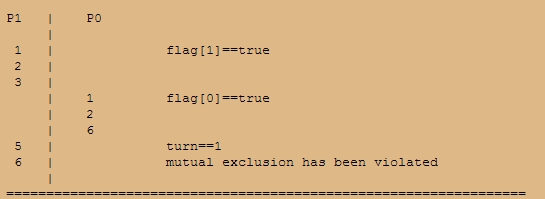
\includegraphics[width=1\textwidth]{scenario.png}
\end{frame}

\end{document}

